\documentclass[10pt,a4paper]{article}

% ---------------------------------------------------------------- layout (MDPI-like)
\usepackage[a4paper,top=2.4cm,bottom=2.4cm,left=4.6cm,right=1.6cm,
            marginparwidth=2.6cm,marginparsep=0.4cm,headheight=14pt]{geometry}
\usepackage[T1]{fontenc}
\usepackage{mathpazo}
\usepackage{amsmath,amssymb,bm}
\usepackage{microtype}
\usepackage{graphicx}
\usepackage{booktabs,tabularx,threeparttable}
\usepackage{changepage}
\usepackage[table]{xcolor}
\usepackage{caption}
\usepackage{enumitem}
\usepackage{fancyhdr}
\usepackage{lastpage}
\usepackage{titlesec}
\usepackage[hidelinks]{hyperref}

\definecolor{mdpiblue}{RGB}{0,73,135}
\definecolor{rulegray}{RGB}{150,150,150}
\newlength{\extralength}\setlength{\extralength}{3.0cm}
\newenvironment{widebox}{\begin{adjustwidth}{-\extralength}{0cm}\centering}{\end{adjustwidth}}

\reversemarginpar
\setlength{\parindent}{1.2em}
\setlength{\parskip}{0pt}
\linespread{1.08}
\setlength{\emergencystretch}{3em}

\captionsetup{font=small,labelfont=bf,labelsep=period,justification=justified,singlelinecheck=false}
\captionsetup[table]{position=top,skip=4pt}
\captionsetup[figure]{skip=4pt}

\titleformat{\section}{\normalfont\bfseries}{\thesection.}{0.5em}{}
\titleformat{\subsection}{\normalfont\itshape}{\thesubsection.}{0.5em}{}
\titlespacing*{\section}{0pt}{12pt}{6pt}
\titlespacing*{\subsection}{0pt}{9pt}{4pt}

\pagestyle{fancy}
\fancyhf{}
\fancyheadoffset[L]{\extralength}
\fancyhead[L]{\small\itshape White Paper, Version 2.0 (2026)}
\fancyhead[R]{\small \thepage\ of \pageref{LastPage}}
\renewcommand{\headrulewidth}{0.4pt}
\fancypagestyle{first}{\fancyhf{}\renewcommand{\headrulewidth}{0pt}
  \fancyhead[L]{\textcolor{mdpiblue}{\bfseries\large White Paper}}
  \fancyhead[R]{\small An-Najah National University}}

\newcommand{\Phihat}{\hat{\Phi}}
\newcommand{\pp}{\,\textup{pp}}
\makeatletter\newcommand{\tabinput}[1]{\@@input #1 }\makeatother

\begin{document}
\thispagestyle{first}

% ---------------------------------------------------------------- title block
\begin{adjustwidth}{-\extralength}{0cm}
{\small\textit{Article}}\par\vspace{4pt}
{\Large\bfseries Low-Complexity Piecewise-Linear Approximations of the Standard Normal CDF for Engineering Calculations: An Accuracy-Complexity Analysis\par}
\vspace{10pt}
{\bfseries Ramiz Assaf}\par\vspace{4pt}
{\small Department of Industrial Engineering, An-Najah National University, Nablus, Palestine;\\
ramizassaf@najah.edu}
\end{adjustwidth}

\marginpar{\raggedright\scriptsize
\vspace{1.2cm}
\textbf{Citation:} Assaf, R. Low-Complexity Piecewise-Linear Approximations of the Standard Normal CDF for Engineering Calculations: An Accuracy-Complexity Analysis. White Paper v2.0; An-Najah National University, 2026.\\[8pt]
\textbf{Code and data:} github.com/\allowbreak ramizassaf/\allowbreak normal-cdf-\allowbreak piecewise-linear\\[8pt]
\textbf{Version:} 2.0 (revised after review), October 2026\\[8pt]
\textbf{Copyright:} \copyright\ 2026 by the author. Distributed under the terms of the Creative Commons Attribution (CC BY 4.0) license.}

\vspace{10pt}
\noindent\textbf{Abstract:} Engineers still evaluate the standard normal cumulative distribution function $\Phi(z)$ by hand when checking software output, teaching, or working without statistical tools. This paper evaluates piecewise-linear approximations of $\Phi(z)$ on $0 \le z \le 3$ as an accuracy-complexity problem. Six three-segment models are compared: exact-secant interpolation through $\Phi(0),\ldots,\Phi(3)$; the rounded-coefficient version used in an earlier draft; a continuous two-digit model (0.50, 0.84, 0.98, 1.00); and three models obtained by solving a minimax linear programme with integer, free, and simplicity-constrained breakpoints. All statistics are computed on a 30{,}001-point grid against a reference CDF verified to $1.1\times10^{-16}$. Exact-secant interpolation underestimates $\Phi$ everywhere inside each segment, as concavity predicts, with maximum absolute error 0.0240 (2.40 percentage points) at $z = 1.47$. Minimax node values at the same integer breakpoints reduce this to 0.0139, and free breakpoints to 0.0092. Counting stored constants as the complexity measure, equal-width breakpoints with minimax node values dominate free breakpoints up to seven constants. Errors of one to two percentage points in $\Phi$ translate into relative errors of 35\% to 150\% in tail probabilities between $z = 1.5$ and $z = 2.8$. These approximations therefore suit rough coverage and yield estimates, and do not suit defect-rate (ppm) estimation.

\vspace{6pt}
\noindent\textbf{Keywords:} normal distribution; piecewise-linear approximation; minimax approximation; linear programming; accuracy-complexity trade-off; process capability; engineering education

\vspace{8pt}
\noindent\textcolor{rulegray}{\rule{\textwidth}{0.4pt}}

% ================================================================ 1
\section{Introduction}

The standard normal cumulative distribution function (CDF),
\begin{equation}
\Phi(z) = \frac{1}{\sqrt{2\pi}} \int_{-\infty}^{z} e^{-t^{2}/2}\,dt ,
\end{equation}
has no closed form. Statistical software evaluates $\Phi$ to machine precision, so the practical case for a hand approximation rests on three narrower needs: checking software output for gross errors, teaching how approximation error behaves, and working in settings without tools. In each case the user trades accuracy for something easier to remember or compute.

Joining tabulated values of $\Phi$ by straight lines is classical interpolation and is not new. This paper makes three narrower contributions. First, it separates models that earlier drafts mixed together (exact-secant, rounded, and continuous two-digit models) and states their boundary behaviour. Second, it formulates breakpoint and node-value selection as a minimax problem, solves it, and reports an accuracy-complexity frontier with an explicit complexity measure. Third, it quantifies how CDF errors propagate into the tail probabilities that drive defect-rate estimates.

The analysis is restricted to $0 \le z \le 3$. Negative arguments follow from symmetry, $\Phi(-z) = 1 - \Phi(z)$. Applications with $z > 3$ or with small tail probabilities need exact evaluation.

% ================================================================ 2
\section{Background}

Abramowitz and Stegun~[1] collect rational and polynomial approximations to $\Phi$, including formula 26.2.17 with absolute error below $7.5\times10^{-8}$. Hastings~[2] developed many of these approximations for early digital computers. P\'olya~[3] gave the one-line formula $\Phi(z) \approx \tfrac12 + \tfrac12\sqrt{1-\exp(-2z^{2}/\pi)}$. Bowling et al.~[4], writing for an industrial engineering audience, proposed a logistic approximation with maximum error below $1.4\times10^{-4}$. Modern libraries use algorithms of the Cody or Cephes family for $\Phi$, and Wichura~[5] for its inverse.

These formulas require an exponential and sometimes a square root, so they suit a calculator but not mental arithmetic. Piecewise-linear models need only multiplication and addition. Their error follows the classical bound for linear interpolation~[6]: on a segment of width $h$,
\begin{equation}\label{eq:bound}
|e(z)| \le \frac{h^{2}}{8}\max |\Phi''(z)| .
\end{equation}
With $\Phi''(z) = -z\phi(z)$, whose magnitude peaks at $z=1$ with value $\phi(1) = 0.2420$, the bound for $h = 1$ is 0.0302.

Applications in quality engineering use $\Phi$ for process yield and capability~[7] and for statistical tolerance analysis~[8].

% ================================================================ 3
\section{Notation and Error Metrics}

Let $\Phihat(z)$ denote an approximation. All errors are stated in probability units unless marked otherwise.

\begin{itemize}[leftmargin=1.4em,itemsep=2pt]
\item Signed error: $e(z) = \Phihat(z) - \Phi(z)$. Negative values mean underestimation.
\item Absolute error: $|e(z)|$. A value of 0.0240 equals 2.40 percentage points (pp); the conversion is $100\,|e|$ pp.
\item Relative CDF error: $100\,|e(z)|/\Phi(z)$, in percent.
\item Tail probability $Q(z) = 1 - \Phi(z)$ and its relative error $r_Q(z) = 100\,(\hat{Q}-Q)/Q$, in percent, with $\hat{Q} = 1-\Phihat$.
\item Two-sided coverage of a centred symmetric interval: $P(|Z|\le z) = 2\Phi(z) - 1$. Its error is $2e(z)$, double the CDF error.
\end{itemize}

Statistics are evaluated on $z = 0, 0.0001, \ldots, 3$ (30{,}001 points). The reference $\Phi$ is \texttt{scipy.special.ndtr}~[9], checked against 50-digit \texttt{mpmath}~[10] at 3{,}001 points; the largest difference is $1.1\times10^{-16}$.

% ================================================================ 4
\section{Three Interpolation-Based Models}

\subsection{Model A: exact secant}

Model A joins $(k,\Phi(k))$, $k = 0,1,2,3$, with straight lines, using unrounded values (Table~\ref{tab:bp}):
\begin{equation}
\Phihat_A(z) = \Phi(k) + m_k\,(z-k), \quad k \le z \le k+1, \quad m_k = \Phi(k+1)-\Phi(k).
\end{equation}
Model A is continuous by construction.

\begin{table}[h]
\caption{Breakpoint values and exact secant slopes used by Model A.}\label{tab:bp}
\centering\small
\begin{tabular}{cccc}
\toprule
$k$ & $\Phi(k)$ & Segment & Slope $m_k$\\
\midrule
\tabinput{tables/tab_breakpoints.tex}
\bottomrule
\end{tabular}
\end{table}

\textit{Sign of the error.} For $z>0$, $\Phi''(z) = -z\phi(z) < 0$, so $\Phi$ is strictly concave on the whole positive half-axis. A chord of a strictly concave function lies below the function between its end points. Hence $\Phihat_A(z) < \Phi(z)$ inside every segment and $e_A(z) = 0$ only at the breakpoints. Model A underestimates $\Phi$; its errors do not oscillate around zero. The computation confirms this: the largest positive error of Model A is 0.0000 (Table~\ref{tab:summary}).

\subsection{Model B: rounded coefficients, as originally published}

The earlier draft rounded the slopes to two decimals and kept three-decimal intercepts:
\begin{equation}
\Phihat_B(z) =
\begin{cases}
0.50 + 0.34\,z, & 0 \le z \le 1,\\
0.841 + 0.14\,(z-1), & 1 < z \le 2,\\
0.977 + 0.02\,(z-2), & 2 < z \le 3.
\end{cases}
\end{equation}
Model B is discontinuous. With the closed-right convention above, Table~\ref{tab:bnd} lists the behaviour at each interior breakpoint. The jump at $z=2$ is $-0.004$, and just left of $z=2$ Model B overestimates $\Phi$ by $+0.0038$, so rounding breaks the one-sided error property of Model A. We report Model B for completeness and do not recommend it.

\begin{table}[h]
\caption{Boundary behaviour of Model B at its interior breakpoints.}\label{tab:bnd}
\centering\small
\begin{tabular}{cccccc}
\toprule
$z$ & $\Phi(z)$ & $\Phihat_B(z)$ & Right limit & Jump & $e_B(z)$\\
\midrule
1 & 0.8413 & 0.840 & 0.841 & $+0.001$ & $-0.0013$\\
2 & 0.9772 & 0.981 & 0.977 & $-0.004$ & $+0.0038$\\
\bottomrule
\end{tabular}
\end{table}

\subsection{Model C: continuous two-digit nodes (``50-84-98-100'')}

Model C keeps the slopes 0.34, 0.14 and 0.02 but chains the intercepts so the function is continuous:
\begin{equation}
\Phihat_C(z) =
\begin{cases}
0.50 + 0.34\,z, & 0 \le z \le 1,\\
0.84 + 0.14\,(z-1), & 1 < z \le 2,\\
0.98 + 0.02\,(z-2), & 2 < z \le 3.
\end{cases}
\end{equation}
The four node values 0.50, 0.84, 0.98 and 1.00 are easy to recall because $\Phi(1)$ and $\Phi(2)$ follow from the 68-95 rule: $\Phi(1) = (1+0.6827)/2$ and $\Phi(2) = (1+0.9545)/2$. Model C overestimates near $z=2$ and at $z=3$, where $\Phihat_C(3) = 1.00$ forces the tail estimate to zero.

\begin{table}[h]
\caption{Values and signed errors of Models A, B and C at selected points.}\label{tab:pts}
\centering\small
\begin{tabular}{cccccccc}
\toprule
$z$ & $\Phi(z)$ & $\Phihat_A$ & $e_A$ & $\Phihat_B$ & $e_B$ & $\Phihat_C$ & $e_C$\\
\midrule
\tabinput{tables/tab_points.tex}
\bottomrule
\end{tabular}
\end{table}

Table~\ref{tab:pts} shows the trap in checking only half-integer points: Model A's largest error on $[0,3]$ occurs at $z = 1.47$ ($-0.0240$), not at $z = 0.5$ ($-0.0208$). The local maximum on the first segment is $-0.0211$ at $z = 0.56$. All three values sit below the bound of Equation~(\ref{eq:bound}).

% ================================================================ 5
\section{Optimisation Formulation}

For $k$ segments with breakpoints $0 = b_0 < b_1 < \cdots < b_k = 3$ and node values $y_0,\ldots,y_k$, let $L(z;\mathbf{b},\mathbf{y})$ be the continuous piecewise-linear function through $(b_j, y_j)$. The design problem is
\begin{equation}\label{eq:opt}
\min_{\mathbf{b},\,\mathbf{y}} \; \max_{0\le z\le 3} \big|L(z;\mathbf{b},\mathbf{y}) - \Phi(z)\big|
\quad\text{s.t.}\quad y_0 = 0.5,\;\; 0 \le y_j \le 1 .
\end{equation}
The constraint $y_0 = 0.5$ keeps the symmetric extension $\Phihat(-z) = 1-\Phihat(z)$ continuous at zero, and the bounds keep $\Phihat$ a valid probability. Continuity is built into $L$. Monotonicity was not imposed; every solution reported below satisfies it.

For fixed $\mathbf{b}$, problem~(\ref{eq:opt}) on the grid is a linear programme in $(\mathbf{y}, t)$: minimise $t$ subject to $-t \le L(z_i) - \Phi(z_i) \le t$ at every grid point. We solve it with the HiGHS solver~[11] through SciPy. Free breakpoints are found by an outer Nelder-Mead search~[12] with seven starting points. The outer search is local, so free-breakpoint results are the best found, not proven global optima. Three solutions are reported:

\begin{itemize}[leftmargin=1.4em,itemsep=2pt]
\item \textbf{Model D}: integer breakpoints, minimax node values (the linear programme alone).
\item \textbf{Model E}: free breakpoints, minimax node values.
\item \textbf{Model F}: simplicity-constrained optimum. Breakpoints are restricted to multiples of 0.5 and node values to two decimals; all combinations within $\pm0.02$ of the continuous optimum are searched exhaustively.
\end{itemize}

\begin{table}[h]
\caption{Optimised three-segment models (breakpoints and node values rounded to four decimals for display; full precision in \texttt{results.json}).}\label{tab:opt}
\centering\small
\begin{tabular}{llll}
\toprule
Model & Breakpoints $\mathbf{b}$ & Node values $\mathbf{y}$ & Max $|e|$\\
\midrule
\tabinput{tables/tab_optimised.tex}
\bottomrule
\end{tabular}
\end{table}

Model F lands on integer breakpoints with node values 0.50, 0.85, 0.99, 0.99. Its last segment is flat, which minimises the CDF error but gives a poor tail (Section~\ref{sec:tail}). Rounding Model E's constants to four decimals raises its maximum error from 0.00923 to 0.00928.

% ================================================================ 6
\section{Results}

\subsection{Error statistics}

\begin{table}[h]
\caption{Error statistics on $0 \le z \le 3$ (30{,}001 points). Columns 2 to 8 in probability units; multiply by 100 for percentage points.}\label{tab:summary}
\begin{widebox}\small
\begin{tabular}{lcccccccc}
\toprule
Model & Max $|e|$ & at $z$ & Mean $e$ & Mean $|e|$ & RMSE & 95th pct $|e|$ & Max $e>0$ & Max rel. (\%)\\
\midrule
\tabinput{tables/tab_summary.tex}
\bottomrule
\end{tabular}
\end{widebox}
\end{table}

\begin{figure}[h]
\begin{widebox}
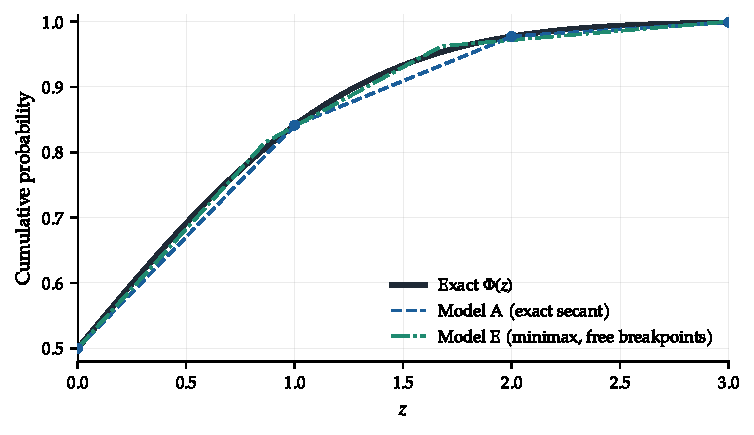
\includegraphics[width=0.78\linewidth]{figures/fig1_cdf.pdf}
\end{widebox}
\caption{Exact $\Phi(z)$, Model A (exact secant through the dots) and Model E (minimax with free breakpoints).}\label{fig:cdf}
\end{figure}

\begin{figure}[h]
\begin{widebox}
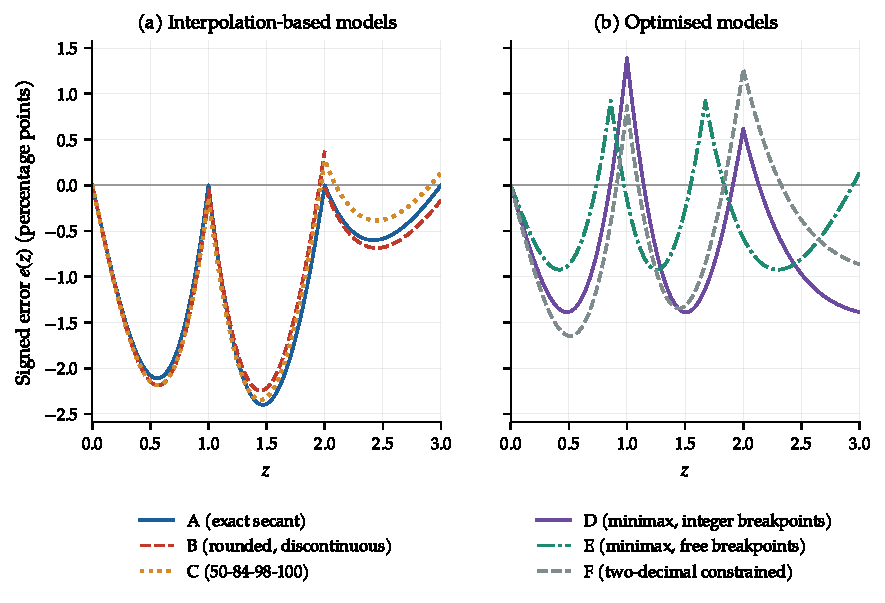
\includegraphics[width=0.95\linewidth]{figures/fig2_error.pdf}
\end{widebox}
\caption{Signed error $e(z)$ in percentage points. (a) Interpolation-based models: Model A stays at or below zero, consistent with concavity; Model B jumps at $z=1$ and $z=2$. (b) Optimised models equalise positive and negative peaks, which is the signature of a minimax solution.}\label{fig:err}
\end{figure}

Three results stand out in Table~\ref{tab:summary} and Figure~\ref{fig:err}. Model A's mean signed error equals minus its mean absolute error, confirming one-sided underestimation; earlier drafts reported a mean error near zero, which was incorrect. Rounding (Models B and C) changes the maximum error by less than 0.002 but introduces overestimation. Choosing node values by minimax (Model D) cuts the maximum error by 42\% with the same integer breakpoints and the same arithmetic effort.

\subsection{Accuracy-complexity frontier}

We measure complexity as the number of constants a user must store. Equal-width models store $k+1$ node values (breakpoints are implied); free-breakpoint models also store $k-1$ interior breakpoints, for $2k$ constants in total. Table~\ref{tab:front} and Figure~\ref{fig:front} report the best maximum error found for $k = 1,\ldots,6$.

\begin{table}[h]
\caption{Maximum absolute error by number of segments $k$ and number of stored constants.}\label{tab:front}
\centering\small
\begin{tabular}{cccccc}
\toprule
 & \multicolumn{3}{c}{Equal-width breakpoints} & \multicolumn{2}{c}{Free breakpoints}\\
\cmidrule(lr){2-4}\cmidrule(lr){5-6}
$k$ & Constants & Interpolation & Minimax values & Constants & Minimax values\\
\midrule
\tabinput{tables/tab_frontier.tex}
\bottomrule
\end{tabular}
\end{table}

\begin{figure}[h]
\centering
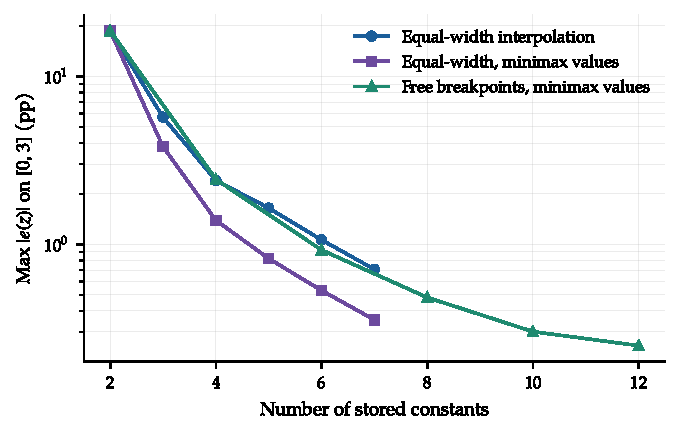
\includegraphics[width=0.72\linewidth]{figures/fig3_frontier.pdf}
\caption{Accuracy-complexity frontier. For a fixed number of stored constants, equal-width breakpoints with minimax node values give the smallest error in this study.}\label{fig:front}
\end{figure}

Two conclusions follow, both conditional on this complexity measure. Per segment, free breakpoints give the smallest error. Per stored constant, equal-width breakpoints with minimax node values dominate: four constants give 0.0139, while free breakpoints need six constants to reach 0.0092 and eight to reach 0.0048. The earlier draft claimed that six equal-width interpolation segments give a maximum error near 0.0005; the computed value is 0.0071, and that claim is withdrawn.

The frontier is a frontier of the models computed here. Human effort also depends on the arithmetic (multiplying by 0.34 versus 0.3655), which the constant count does not capture. A study with users would be needed to measure that cost.

\subsection{Reference non-linear approximations}

Table~\ref{tab:ref} places the linear models in context. P\'olya's formula reaches 0.0031 with a single expression, an order of magnitude better than any three-segment linear model, at the cost of an exponential and a square root.

\begin{table}[h]
\caption{Classical closed-form approximations evaluated on the same grid.}\label{tab:ref}
\centering\small
\begin{tabular}{lccl}
\toprule
Approximation & Max $|e|$ & at $z$ & Operations\\
\midrule
\tabinput{tables/tab_reference.tex}
\bottomrule
\end{tabular}
\end{table}

\subsection{Tail probabilities}\label{sec:tail}

Defect rates depend on $Q(z) = 1-\Phi(z)$, which is small exactly where the CDF error looks small. Table~\ref{tab:tail} reports two-sided out-of-specification rates, $2Q(z)\times10^{6}$ ppm, for a centred process.

\begin{table}[h]
\caption{Two-sided defect rates (ppm) and relative tail error $r_Q$ (\%) for a centred process.}\label{tab:tail}
\begin{widebox}\small
\begin{tabular}{cccccccc}
\toprule
$z$ & Exact ppm & Model A ppm & $r_Q$ A & Model C ppm & $r_Q$ C & Model E ppm & $r_Q$ E\\
\midrule
\tabinput{tables/tab_tail.tex}
\bottomrule
\end{tabular}
\end{widebox}
\end{table}

\begin{figure}[h]
\begin{widebox}
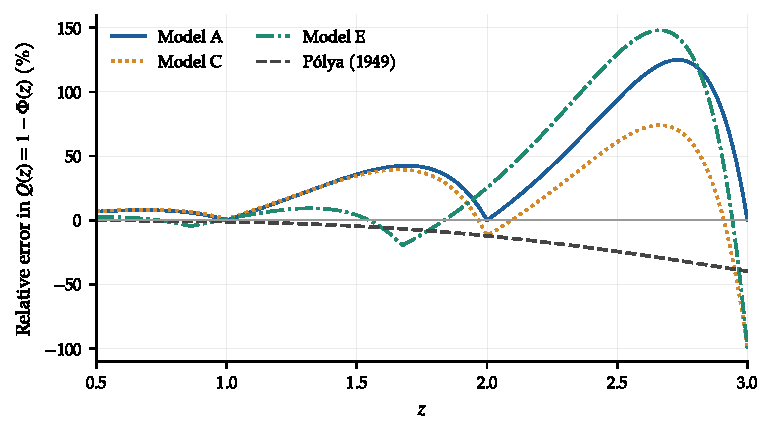
\includegraphics[width=0.78\linewidth]{figures/fig4_tail.pdf}
\end{widebox}
\caption{Relative error in the tail probability $Q(z)$. Errors below 2.5 percentage points in $\Phi$ become tail errors of 35\% to 150\%. Model C and Model E return $\hat{Q}(3) = 0$, a relative error of $-100\%$.}\label{fig:tail}
\end{figure}

At $z = 2.5$, Model A's CDF error is only $-0.0058$, yet it reports 24{,}100 ppm instead of 12{,}419 ppm, an overestimate of 94\%. The minimax models do not fix this: Model E is optimal for the CDF and still overestimates the tail at $z=2.5$ by 130\%. A model meant for defect rates needs a different objective, for example minimax relative error in $Q$.

% ================================================================ 7
\section{Engineering Examples}

\subsection{Centred process yield}

A bearing diameter has specification limits $\pm0.050$\,mm around nominal, process standard deviation $\sigma = 0.020$\,mm, and a centred mean. The distance to each limit is $z = 0.050/0.020 = 2.5$, so $C_p = 0.100/(6\times0.020) = 0.833$. Two-sided yield is $2\Phi(2.5)-1$.

\begin{itemize}[leftmargin=1.4em,itemsep=2pt]
\item Exact: $\Phi(2.5) = 0.99379$; yield 98.758\%; 12{,}419 ppm out of specification.
\item Model A: $\Phihat_A(2.5) = 0.98795$; yield 97.590\% ($-1.17$\pp); 24{,}100 ppm ($+94\%$).
\item Model C: $\Phihat_C(2.5) = 0.99$; yield 98.000\% ($-0.76$\pp); 20{,}000 ppm ($+61\%$).
\end{itemize}

The yield estimates are within about one percentage point. The ppm estimates are off by a factor between 1.6 and 1.9.

\subsection{One-sided versus two-sided probability}

The probability of conformance to a bilateral tolerance $\pm T$ with stack-up standard deviation $\sigma$ is $P(|Z|\le T/\sigma) = 2\Phi(T/\sigma)-1$, not $\Phi(T/\sigma)$. For $T/\sigma = 1.2$, the exact value is $2(0.88493)-1 = 0.76986$. Model C gives $\Phihat_C(1.2) = 0.84 + 0.14(0.2) = 0.868$ and a coverage of 0.736, an error of $-3.39$\pp, double its CDF error of $-1.69$\pp.

\subsection{Outside the range}

A centred process with $C_{pk} = 1.33$ has $z = 3C_{pk} \approx 4$. The exact two-sided yield is 99.9937\% (63 ppm). This lies outside $[0,3]$ and none of the models here applies.

% ================================================================ 8
\section{Quick Field Rules}

For use without tables, a calculator, or software, Model C reduces to four remembered numbers and three slopes.

\begin{enumerate}[leftmargin=1.6em,itemsep=2pt]
\item Remember the nodes 0.50, 0.84, 0.98 at $z = 0, 1, 2$ (from the 68-95 rule) and 1.00 at $z = 3$.
\item Find the segment containing $|z|$ and add slope $\times$ distance: 0.34 on $[0,1]$, 0.14 on $[1,2]$, 0.02 on $[2,3]$.
\item For negative $z$, use $1 - \Phihat(|z|)$. For two-sided coverage, use $2\Phihat - 1$.
\end{enumerate}

Corrected worked examples (exact values in parentheses): $z=0.5$ gives 0.670 (0.6915, $-2.15$\pp); $z=1.5$ gives 0.910 (0.9332, $-2.32$\pp); $z=1.8$ gives 0.952 (0.9641, $-1.21$\pp); $z=2.5$ gives 0.990 (0.9938, $-0.38$\pp).

\textit{When a calculator is available}, P\'olya's formula reduces the maximum error to 0.0031 with one line and no table.

\textit{Suitability.} Model C keeps $|e| \le 0.0235$ on $[0,3]$, so two-sided coverage stays within $\pm4.7$\pp. These rules suit decisions that do not change within that band, such as rough yield screening, sanity checks of software output, and classroom estimation. They do not suit ppm or defect-rate estimates, capability claims near specification limits, safety-critical reliability, or any $z > 3$.

Table~\ref{tab:def} lists exact reference values for common $z$ values, for a centred process without the 1.5$\sigma$ shift convention of Six Sigma practice. This table corrects the earlier draft, in which four of the six ppm entries were wrong.

\begin{table}[h]
\caption{Exact reference values for a centred process (no 1.5$\sigma$ shift).}\label{tab:def}
\centering\small
\begin{tabular}{ccccc}
\toprule
$z$ & $\Phi(z)$ & Two-sided coverage (\%) & Two-sided ppm & One-sided ppm\\
\midrule
\tabinput{tables/tab_defects.tex}
\bottomrule
\end{tabular}
\end{table}

% ================================================================ 9
\section{Implementation}

A spreadsheet version of Model C, symmetric for negative $z$ and returning \texttt{\#N/A} outside $[-3,3]$ (cell \texttt{A2} holds $z$):

\begin{center}
\fcolorbox{rulegray}{gray!6}{\begin{minipage}{0.95\linewidth}\footnotesize\ttfamily\raggedright
=IF(ABS(A2)>3,NA(),0.5+SIGN(A2)*IF(ABS(A2)<=1,0.34*ABS(A2),\\
\hspace*{2em}IF(ABS(A2)<=2,0.34+0.14*(ABS(A2)-1),0.48+0.02*(ABS(A2)-2))))
\end{minipage}}
\end{center}

\noindent Enter the formula as a single line; a copy is in \texttt{spreadsheet/model\_C\_formula.txt} in the repository. The formula reproduces Model C and its symmetric extension to within $1.1\times10^{-16}$ on 601 test points in $[-3,3]$. Returning \texttt{\#N/A} outside the range is deliberate: silent extrapolation would produce probabilities above one. The repository also contains Python reference code and an interactive browser application that plots all models, their errors and the tail effect, and computes yield and ppm for user-supplied specification limits.

% ================================================================ 10
\section{Limitations}

The minimax problem is solved on a discrete grid with step $10^{-4}$; the continuous optimum can differ slightly. Free breakpoints come from a local search with multiple starts, so better solutions may exist. The complexity measure counts constants and ignores arithmetic difficulty and memory errors; no user study was performed. All objectives concern absolute CDF error on $[0,3]$; a tail-weighted or relative-error objective would produce different models and is left for future work.

% ================================================================ 11
\section{Conclusions}

Piecewise-linear approximation of $\Phi(z)$ on $[0,3]$ is a classical idea; its value lies in a clear statement of what it can and cannot do. Exact-secant interpolation through integer points underestimates $\Phi$ with a maximum error of 0.0240 at $z = 1.47$. Choosing node values by minimax at the same breakpoints reduces this to 0.0139 at no extra effort, and free breakpoints reach 0.0092. Measured by stored constants, equal-width breakpoints with minimax node values give the best trade-off among the models computed. The continuous two-digit Model C (0.50, 0.84, 0.98, 1.00) is the most memorable option, with a maximum error of 0.0235. For all linear models, errors of one to two percentage points in $\Phi$ become errors of tens of percent in tail probabilities, so these tools serve rough yield and coverage estimates and should not replace exact computation of defect rates.

\vspace{10pt}
\noindent\textcolor{rulegray}{\rule{\textwidth}{0.4pt}}
\small

\vspace{4pt}\noindent\textbf{Author Contributions:} Conceptualization, methodology, validation, writing (review and editing), R.A. The author has read and agreed to the published version of the manuscript.

\vspace{4pt}\noindent\textbf{Funding:} This research received no external funding.

\vspace{4pt}\noindent\textbf{Data Availability Statement:} All code, the full error grid and every reported statistic are available at \url{https://github.com/ramizassaf/normal-cdf-piecewise-linear}. Running \texttt{analysis/compute\_results.py} regenerates all numbers in this paper.

\vspace{4pt}\noindent\textbf{Acknowledgments:} This white paper was prepared with the help of Claude, an AI assistant developed by Anthropic. Claude Haiku 4.5 assisted with the first draft. Claude Opus 5.5 carried out the technical review for this revision: it recomputed every reported statistic, implemented and solved the optimisation models, produced the figures, corrected errors in the first draft, and built the interactive application. The author directed the work, reviewed all content, and takes full responsibility for it. The author thanks Anthropic for making these tools available, and thanks the anonymous reviewer whose comments shaped this revision.

\vspace{4pt}\noindent\textbf{Conflicts of Interest:} The author declares no conflicts of interest.

\vspace{4pt}\noindent\textbf{Revision note:} Version 1 of this white paper contained numerical errors, including the location and size of the maximum error, the boundary values of Model B, the defect-rate table, a six-segment error claim, and validation statistics that had not been computed. Version 2 replaces all of them with values generated by the published code.

\section*{References}
\begin{enumerate}[label={\arabic*.},leftmargin=1.6em,itemsep=1pt]
\item Abramowitz, M.; Stegun, I.A. (Eds.) \textit{Handbook of Mathematical Functions with Formulas, Graphs, and Mathematical Tables}; Applied Mathematics Series 55; National Bureau of Standards: Washington, DC, USA, 1964.
\item Hastings, C. \textit{Approximations for Digital Computers}; Princeton University Press: Princeton, NJ, USA, 1955.
\item P\'olya, G. Remarks on computing the probability integral in one and two dimensions. In \textit{Proceedings of the First Berkeley Symposium on Mathematical Statistics and Probability}; University of California Press: Berkeley, CA, USA, 1949; pp. 63--78.
\item Bowling, S.R.; Khasawneh, M.T.; Kaewkuekool, S.; Cho, B.R. A logistic approximation to the cumulative normal distribution. \textit{J. Ind. Eng. Manag.} \textbf{2009}, \textit{2}, 114--127. https://doi.org/10.3926/jiem.2009.v2n1.p114-127
\item Wichura, M.J. Algorithm AS 241: The percentage points of the normal distribution. \textit{J. R. Stat. Soc. Ser. C Appl. Stat.} \textbf{1988}, \textit{37}, 477--484.
\item de Boor, C. \textit{A Practical Guide to Splines}, revised ed.; Springer: New York, NY, USA, 2001.
\item Montgomery, D.C. \textit{Introduction to Statistical Quality Control}, 8th ed.; Wiley: Hoboken, NJ, USA, 2019.
\item Chase, K.W.; Parkinson, A.R. A survey of research in the application of tolerance analysis to the design of mechanical assemblies. \textit{Res. Eng. Des.} \textbf{1991}, \textit{3}, 23--37.
\item Virtanen, P.; Gommers, R.; Oliphant, T.E.; et al. SciPy 1.0: Fundamental algorithms for scientific computing in Python. \textit{Nat. Methods} \textbf{2020}, \textit{17}, 261--272.
\item Johansson, F.; et al. mpmath: A Python library for arbitrary-precision floating-point arithmetic, version 1.3.0, 2023. Available online: https://mpmath.org
\item Huangfu, Q.; Hall, J.A.J. Parallelizing the dual revised simplex method. \textit{Math. Program. Comput.} \textbf{2018}, \textit{10}, 119--142.
\item Nelder, J.A.; Mead, R. A simplex method for function minimization. \textit{Comput. J.} \textbf{1965}, \textit{7}, 308--313.
\end{enumerate}

\end{document}
